\chapter{Analysis}
Overall, total two objectives are required for the project. In the first part, propose a novel machine learning to modeling different PUF(physical unclonable function)
behavior, in particular arbiter PUF and XOR arbiter PUF. In the second part, consider reconfigurability like adding noise, one-time-PUF to resilient against the modeling attack
proposed in part one.

\section{Project Aims and Evaluation}
The aims for part one are that the machine learning for modeling should be related to ETA(estimated time arrival) problem or the one people haven't used for modeling
PUF. Moreover, reconfigurability need to be considered when proposing the modeling attack while knowing the PUF can escape from it by changing CRPs behaviors in part 
two. Therefore, the machine learning should ideally adapt to the changing behavior of CRPs or the PUF. For example, unsupervised learning can be a good way since it can 
deal with unseen data. To evaluate the work, an overall accuracy of the modeling are expected to be around 90\% and take short time like the logistic regression in 
paper \cite{Reference6}.

The aims for part two are proposing a reconfigurability framework for the modeling attack in part one. Two different reconfigurability will be implemented. First, add intentional
noise to PUF's response during authentication phase to disturb the modeling attack \cite{Reference8}. The basic idea is shown in Figure \ref{fig:figure10}, assume database has stored PUF's CRPs and provide a challenge c
to PUF in authentication phase. The PUF return a response r', and add noise e with r'. Then e and r' compose helper data h and send back to verifier, where $h = r'\oplus e$. The verifier can reproduce $r'\oplus e$  
with r and h if r and $r'\oplus e$ is similar. Last, both verifier and user create their own hashtag and compare to check if authenticate. In this case, attacker only access to c and $r'\oplus e$, which the modeling
will not be accurate unless the attacker's model response is closed enough to r'.

\begin{figure}[htp]
    \centering
    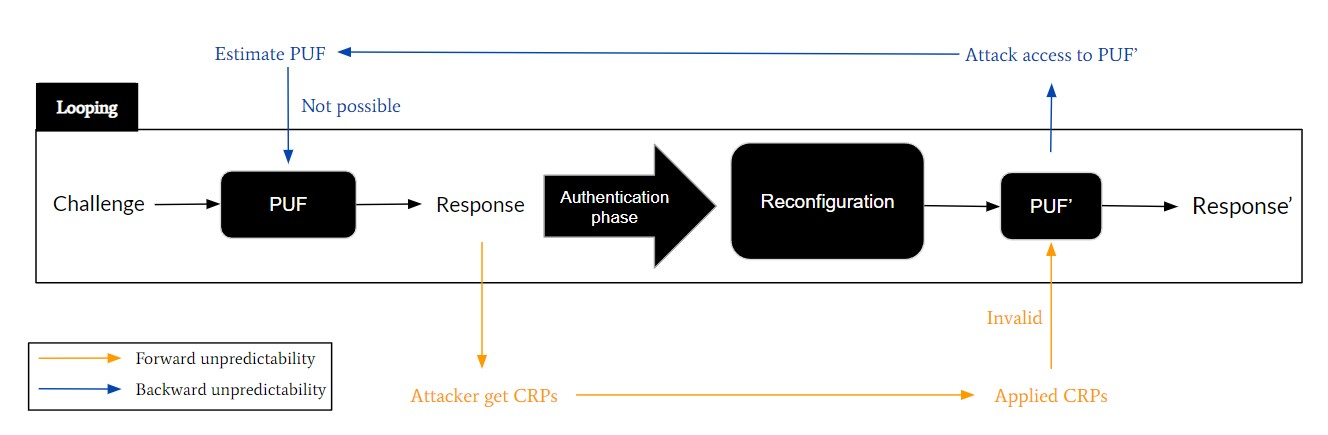
\includegraphics[width=14cm]{figures/figure8.jpg}
    \caption{Add noise to PUF's response during authentication phase}
    \label{fig:figure10}
    \end{figure}
Second, implement OPUF to change the behavior of CRPs.

To evaluate the work, the modeling attack proposed in part one should have reasonable accuracy drop and the authentication will still work though noise is added.



\section{Ethical, Professional and Legal Issues}


